In this chapter is explained the case of study inside the D-DUST project, paying attention on the data used in the different period, resolution and target variable. 

\section{Data sets description}
This case of study aims to discover the main factors which affects mostly the target variable chosen. 
Variables selected are the physical and chemical factors that are most associated with the formation of primary and secondary pollutant. \newline
Therefore, the variables are categorized in 4 different labels:
\begin{itemize}
\item Weather: These elements, such as wind speed and direction, precipitation and air temperature, changes in the epochs and can influence air pollution;
\item Pollutant: These variables represent primary and secondary pollutant related to the greenhouse effect;
\item Soil and Vegetation: Since soil and vegetation degradation are global concerns and can influence the air propagation in the environment, data related to local morphology are collected;
\item GIS (time invariant layers): This time-invariant layers are considered to be changeless in the time range considered. Differently from the other types which need a constant monitoring, these variables are update yearly with a lower frequency than the others;
\end{itemize}
Data chosen are open source and regularly available.
In this phase data have been collected (not by me but by other colleagues of D-DUST project at this \underline{ \href{https://docs.google.com/spreadsheets/d/1-5pwMSc1QlFyC8iIaA-l1fWhWtpqVio2/edit\#gid=91313358}{link}}) in grids from different sources and provided in geopackages. 
\subsection{Source types}
In order to better distinguish the data sources characteristics, variables selected are labelled with 4 different types of source:
\begin{itemize}

\item Ground Sensor: Each ground monitoring stations which provide meteorological and air quality data belongs mainly to: 
\begin{itemize}
    \item ARPA (Agenzia Regionale per la Prevenzione dell'Ambiente);
    \item ESA Air Quality Platform (low cost sensor)\cite{esasensor};
\end{itemize}  
\item Model: data are estimated through a model built using satellite and meteorological and air quality data as input, such as European data provided by CAMS (Copernicus Atmosphere Monitoring Service);
\item Map layer: this data are time-invariant and are related to Lombardy morphology such as density of roads, population or land use; 
\item Satellite Sensor: They provide data from air quality observation mainly. Satellites provider are Sentinel-5P Tropomi and Terra \& Aqua MODIS;
\end{itemize}
\bigbreak

In the next lines each variable is provided in tables, by showing its type, name and description:

\subsection{Meteo Variable (Table)}
\begin{center}
\setlength{\arrayrulewidth}{1.5pt}

\begin{longtable}{ |p{2cm}|p{1.5cm}|p{2.3cm}|p{4cm}|p{1cm}|p{2cm}| } 
\hline
\textbf{Physical variable} & \textbf{Source type}  & \textbf{Variable name}  & \textbf{Description}  & \textbf{Unit}  & \textbf{Source}\\ 
\hline
\multirow{3}{4em}{Temperature} & Model  & \underline{temp\_2m} & Mean air temperature at 2 m above the land surface.\par & K & ERA5-Land hourly data.\\ 
& Ground \newline Sensor  & \underline{temp\_lcs} &  Mean air temperature ground measurement - Low Cost Sensor ESA monitoring stations.\par & °C & ESA Air Quality Platform.\\ 
& Ground \newline Sensor  & \underline{temp\_st} &  Mean temperature - ARPA monitoring stations.\par & °C & ARPA \newline Lombardia.\\ \hline
\pagebreak
\hline
\multirow{4}{4em}{Wind} & Model  & \underline{e\_wind} & Mean eastward wind component 10 m above the land surface.\par & m/s & ERA5-Land hourly data.\\ 
& Ground \newline Sensor  & \underline{n\_wind} &  Mean northward wind component 10 m above the land surface.\par & m/s & ERA5-Land hourly data.\\
& Ground \newline Sensor  & \underline{wind\_speed\_st} &  Mean wind speed on ground  - ARPA monitoring stations. \par& m/s& ARPA \newline Lombardia.\\ \hline

\multirow{2}{4em}{Precipitation} & Model  & \underline{prec} & Mean accumulated liquid and frozen water, including rain and snow, that falls to the Earth's surface. It is the sum of large-scale precipitation. \par & mm & ERA5-Land hourly data.\\ 
& Ground \newline Sensor  & \underline{prec\_st} &  Mean precipitation in each cell in the time range - ARPA monitor stations. \par & mm & ARPA \newline Lombardia.\\ \hline

\multirow{2}{4em}{Air Humidity} & Ground \newline Sensor  & \underline{air\_hum\_st} & Mean air moisture measurement in the time range - ARPA monitoring stations.\par & \% & ARPA \newline Lombardia.\\ 
& Ground \newline Sensor  & \underline{air\_hum\_lcs} &  Mean air moisture ground measurement - Low Cost Sensor ESA monitoring stations.\par & \% & ESA Air Quality Platform.\\ \hline

\multirow{1}{4em}{Air Pressure} & Model   & \underline{press} & Mean weight of all the air in a column vertically above the area of the Earth's surface represented at a fixed point.\par & Pa & ERA5-Land hourly data.\\ \hline

\multirow{1}{4em}{Solar Radiation} & Ground \newline Sensor  & \underline{press} & Global radiation measurement - ARPA monitoring station.\par & W/m\textsuperscript{2} & ARPA \newline Lombardia.\\ \hline

\hline
\caption{Table of Meteorological variables.}

\end{longtable}
\end{center}

\subsection{Pollutants Variables (Table)}


\begin{center}
\setlength{\arrayrulewidth}{1.5pt}
\begin{longtable}{ |p{2cm}|p{1.5cm}|p{2.3cm}|p{4cm}|p{1cm}|p{2cm}| } 
\hline
\textbf{Physical variable} & \textbf{Source type}  & \textbf{Variable name}  & \textbf{Description}  & \textbf{Unit}  & \textbf{Source}\\ 
\hline
\multirow{1}{4em}{Dust} & Model  & \underline{dust} & Mean dust concentration at 0m level provided by CAMS (Ensemble Median - Analysis).\par & ug/m\textsuperscript{3} & CAMS Model.\\ \hline

\multirow{3}{4em}{AOD} & Satellite \newline Sensor  & \underline{aod\_055} & Mean Aerosol Optical Depth at 550nm.\par & - & MODIS Terra+Aqua.\\ 
& Satellite \newline Sensor  & \underline{aod\_047} &  Mean Aerosol Optical Depth at 470nm.\par & - & MODIS Terra+Aqua.\\ 
& Satellite \newline Sensor & \underline{uvai} &  Mean UV Aerosol Index. A positive index highlights the presence of UV absorbing aerosol (such as smoke/dust). \par & - & Sentinel-5P\\ \hline

\multirow{3}{4em}{PM10} & Model  & \underline{pm10\_cams} & Mean PM10 concentration at 0m level provided by CAMS  (Ensemble Median - Analysis).\par & ug/m\textsuperscript{3} & CAMS Model.\\ 
& Ground \newline Sensor  & \underline{pm10\_lcs} &  Mean PM10 concentration ground measurement - Low Cost Sensor ESA monitoring stations.\par & not\newline defined & ESA Air Quality Platform.\\ 
& Ground \newline Sensor & \underline{pm10\_st} &  Mean PM10 concentration ground measurement - ARPA monitoring stations. \par & ug/m\textsuperscript{3} & ARPA \newline Lombardia\\ \hline

\multirow{3}{4em}{PM2.5} & Model  & \underline{pm25\_cams} & Mean PM2.5 concentration at 0m level provided by CAMS  (Ensemble Median - Analysis).\par & ug/m\textsuperscript{3} & CAMS Model.\\ 
& Ground \newline Sensor  & \underline{pm25\_lcs} &  Mean PM2.5 concentration ground measurement - Low Cost Sensor ESA monitoring stations.\par & ug/m\textsuperscript{3} & ESA Air Quality Platform.\\ 
& Ground \newline Sensor & \underline{pm25\_st} &  Mean PM2.5 concentration ground measurement - ARPA monitoring stations. \par & ug/m\textsuperscript{3} & ARPA \newline Lombardia\\ \hline
\pagebreak
\hline
\multirow{3}{4em}{SO\textsubscript{2}} & Model  & \underline{so2\_cams} & Mean SO\textsubscript{2} concentration at 0m level provided by CAMS  (Ensemble Median - Analysis).\par & ug/m\textsuperscript{3} & CAMS Model.\\ 
& Satellite \newline Sensor  & \underline{so2\_s5p} &  Mean SO2  vertical column density at ground level. \par& mol/m\textsuperscript{2} & Sentinel-5P.\\ 
& Ground \newline Sensor & \underline{so2\_st} &  Mean SO\textsubscript{2} concentration ground measurement - ARPA monitoring stations. \par & ug/m\textsuperscript{3} & ARPA \newline Lombardia.\\ \hline


\multirow{4}{4em}{NO\textsubscript{2}} & Model  & \underline{no2\_cams} & Mean NO\textsubscript{2} concentration at 0m level provided by CAMS  (Ensemble Median - Analysis).\par & ug/m\textsuperscript{3} & CAMS Model.\\ 
& Satellite \newline Sensor  & \underline{no2\_s5p} &  Mean NO2  vertical column density at ground level.\par & mol/m\textsuperscript{2} & Sentinel-5P.\\ 
& Ground \newline Sensor & \underline{no2\_st} &  Mean NO\textsubscript{2} concentration ground measurement - ARPA monitoring stations. \par & ug/m\textsuperscript{3} & ARPA \newline Lombardia.\\ 
& Ground \newline Sensor & \underline{no2\_lcs} &  Mean NO\textsubscript{2} concentration ground measurement - Low Cost Sensor ESA monitoring stations. \par & ug/m\textsuperscript{3} & ESA Air Quality Platform.\\ \hline

\multirow{1}{4em}{NO} & Model  & \underline{no2\_cams} & Mean NO concentration at 0m level provided by CAMS  (Ensemble Median - Analysis). \par& ug/m\textsuperscript{3} & CAMS Model.\\  \hline

\multirow{1}{4em}{CH\textsubscript{2}O} & Satellite \newline Sensor  & \underline{ch20\_s5p} & Mean Formaldehyde tropospheric column number density. \par& mol/m\textsuperscript{2} & Sentinel-5P.\\  \hline

\multirow{1}{4em}{CH\textsubscript{4}} & Satellite \newline Sensor  & \underline{ch20\_s5p} & Mean column averaged dry air mixing ratio of methane. \par& ppbV & Sentinel-5P.\\  \hline

\multirow{1}{4em}{NO\textsubscript{x}} & Ground \newline Sensor & \underline{nox\_st} &  Mean NO\textsubscript{x} (field: "Ossidi di Azoto") concentration ground measurement - ARPA monitoring stations.\par  & ug/m\textsuperscript{3} & ARPA \newline Lombardia.\\ \hline

\multirow{1}{4em}{CO\textsubscript{2}} & Ground \newline Sensor & \underline{co2\_lcs} &  Mean CO2 concentration ground measurement - Low Cost Sensor ESA monitoring stations. \par & ? & ESA Air Quality Platform.\\ \hline
\pagebreak
\hline
\multirow{4}{4em}{CO} & Model  & \underline{co\_cams} & Mean CO concentration at 0m level provided by CAMS  (Ensemble Median - Analysis).\par & ug/m\textsuperscript{3} & CAMS Model.\\ 
& Satellite \newline Sensor  & \underline{co\_s5p} &  Mean CO vertically integrated column density.\par & mol/m\textsuperscript{2} & Sentinel-5P.\\ 
& Ground \newline Sensor & \underline{co\_st} &  Mean CO concentration ground measurement - ARPA monitoring stations. \par & ug/m\textsuperscript{3} & ARPA \newline Lombardia.\\ 
& Ground \newline Sensor & \underline{co\_lcs} &  Mean CO concentration ground measurement - Low Cost Sensor ESA monitoring stations. \par & ug/m\textsuperscript{3} & ESA Air Quality Platform.\\ \hline

\multirow{3}{4em}{O\textsubscript{3}} & Model  & \underline{o3\_cams} & Mean O\textsubscript{3} concentration at 0m level provided by CAMS  (Ensemble Median - Analysis).\par & ug/m\textsuperscript{3} & CAMS Model.\\ 
& Satellite \newline Sensor  & \underline{03\_s5p} &  Mean O\textsubscript{3} total atmospheric column.\par  & mol/m\textsuperscript{2} & Sentinel-5P.\\ 
& Ground \newline Sensor & \underline{03\_st} &  Mean O\textsubscript{3} concentration ground measurement - ARPA monitoring stations.  \par& ug/m\textsuperscript{3} & ARPA \newline Lombardia.\\ 
 \hline
 
 \multirow{1}{4em}{CH\textsubscript{2}O}& Satellite \newline Sensor  & \underline{ch20\_s5p} &  Mean Formaldehyde tropospheric column number density. \par & mol/m\textsuperscript{2} & Sentinel-5P.\\ \hline
 
\multirow{1}{4em}{NMVOCs}& Model  & \underline{nmvocs\_cams} & Mean Non-Methane VOCs concentrations at 0m level provided by CAMS.\par & ug/m\textsuperscript{3} & CAMS Model.\\ \hline

\multirow{3}{4em}{NH\textsubscript{3}} & Model  & \underline{nh3\_cams} & Mean NH\textsubscript{3} concentration at 0m level provided by CAMS  (Ensemble Median - Analysis).\par & ug/m\textsuperscript{3} & CAMS Model.\\ 
& Satellite \newline Sensor  & \underline{nh3\_lcs} &  Mean NH\textsubscript{3} concentration ground measurement - Low Cost Sensor ESA monitoring stations. \par  & ? & ESA Air Quality Platform.\\ 
& Ground \newline Sensor & \underline{nh3\_st} &  Mean NH\textsubscript{3} concentration ground measurement - ARPA monitoring stations. \par & ug/m\textsuperscript{3} & ARPA \newline Lombardia.\\ \hline
\caption{Table of Pollutant variables.}
\end{longtable}
\end{center}
In addition to them, there's also pollutants variables ending with '\_int' (such as 'pm10\_int', 'pm25\_int', 'nh3\_int', etc.). These variables are obtained by interpolating ARPA variables which are not spatially continued. The explanation of how they are interpolated and how I mitigate the problem of having a limited number of observation from ground sensors along the surface is in one of the next \hyperref[subsec:nan]{subsection}.
\subsection{Soil and Vegetation (Table)}

\begin{center}
\setlength{\arrayrulewidth}{1.5pt}
\begin{longtable}{ |p{2cm}|p{1.5cm}|p{2.3cm}|p{4cm}|p{1cm}|p{2cm}| } 
\hline
\textbf{Physical variable} & \textbf{Source type}  & \textbf{Variable name}  & \textbf{Description}  & \textbf{Unit}  & \textbf{Source}\\ 
\hline

\multirow{3}{4em}{Vegetation} & Satellite \newline Sensor  & \underline{siarlX} & Fraction of area in each cell for each agricultural use provided by SIARL Catalog for Lombardy Region.\par & \% & SIARL Lombardia 2019.\\ 
& Satellite \newline Sensor  & \underline{ndvi} &  Mean NDVI cell value over 16 days period.\par & - & USGS Earth Data.\\ 
& Satellite \newline Sensor  & \underline{siarl} &  Majority class for agricultural use provided by SIARL Catalog for Lombardy Region. \par & cat & SIARL Lombardia 2019.\\
\hline

\multirow{5}{4em}{Soil} & Model  & \underline{soil\_moist} & Mean volume of water in soil layer 1 (0 - 7 cm) of the ECMWF Integrated Forecasting System. The surface is at 0 cm. The volumetric soil water is associated with the soil texture (or classification), soil depth, and the underlying groundwater level.\par & m\textsuperscript{3}/m\textsuperscript{3} & ERA5 Land Hourly Data.\\ 
& Map Layer  & \underline{soilX} &  Fraction of area for each cell containing the soil type obtained from OpenLandMap soil texture classification.\par & \% & OpenLandMap Soil Texture Class (USDA System).\\ 
& Map Layer  & \underline{soil\_textX} &  Mean NDVI cell value over 16 days period. \par & \% & Basi informative dei suoli - Geoportale Lombardia.\\ 
& Map Layer  & \underline{soil} &  Majority soil type for each pixel from OpenLandMap soil texture classification .\par & cat & OpenLandMap Soil Texture Class (USDA System) .\\ 
& Map Layer  & \underline{soil\_text} &  Majority soil type for each pixel from Carta pedologica 250K (Lombardy Region). \par& cat & Basi informative dei suoli - Geoportale Lombardia.\\ 

\hline
\caption{Table of variables referred to Vegetation and Soil.}

\end{longtable}
\end{center}

\subsection{GIS (static layers) (Table)}

\begin{center}
\setlength{\arrayrulewidth}{1.5pt}
\begin{longtable}{ |p{2.1cm}|p{1.5cm}|p{2.3cm}|p{4cm}|p{1.5cm}|p{2cm}| } 
\hline
\textbf{Physical variable} & \textbf{Source type}  & \textbf{Variable name}  & \textbf{Description}  & \textbf{Unit}  & \textbf{Source}\\ 
\hline
\multirow{1}{4em}{Geometry} & Map Layer  & \underline{area} & Area of Lombardy Region vector layer in each cell. \par& km\textsuperscript{2} & SIARL Lombardia 2019.\\ 
\hline
\multirow{1}{4em}{Calendar} & Map Layer  & \underline{cal} & JSON file containing the time-ranges used for data processing. \par& day & -\\ 
\hline

\multirow{1}{4em}{Population} & Map Layer  & \underline{pop} & Population for each cell. & n° of inhabitants& Gridded Population of the World (GPW).\\ \hline

\multirow{2}{4em}{Land use and cover} & Map Layer  & \underline{dsfX} & Land use fraction for each cell containing the classification the classification provided by DUSAF Catalog (Lombardy Region). & \% (fraction for each cell) & DUSAF Lombardia 2018.\\ \hline
Map Layer  & \underline{dusaf} & Cover & Land Use majority class for each cell provided by DUSAF Catalog (Lombardy Region). & cat  & DUSAF Lombardia 2018.\\
\hline

\multirow{3}{4em}{Terrain} & Map Layer  & \underline{h\_mean} & DTM average elevation for each pixel. & m & Geoportale Lombardia 2019.\\ 
& Map Layer  & \underline{aspect\_major} & Aspect derived from DTM. Majority pixel aspect. & Degree North & Geoportale Lombardia 2019.\\ 
& Map Layer  & \underline{slope\_mean} & Average slope derived from DTM. & Degree North & Geoportale Lombardia 2019.\\ 

\hline
\pagebreak
\hline
\multirow{6}{4em}{Road Infrastructures} & Map Layer  & \underline{int\_prim} & Density of intersection nodes between primary roads for each cell (including highways). & int\textsubscript{s}/km\textsuperscript{2} & Geoportale Lombardia 2019.\\ 
& Map Layer  & \underline{int\_prim\_sec} & Density of intersection nodes between primary and secondary roads for each cell. & int\textsubscript{s}/km\textsuperscript{2} & Geoportale Lombardia 2019.\\ 
& Map Layer  & \underline{int\_sec} & Density of intersection nodes between secondary roads for each cell. & int\textsubscript{s}/km\textsuperscript{2} & Geoportale Lombardia 2019.\\ 
& Map Layer  & \underline{prim\_road} & Density of primary importance roads for Lombardy Region inside for each. & km/km\textsuperscript{2} & Geoportale Lombardia 2019.\\ 
& Map Layer  & \underline{sec\_road} & Density of secondary importance roads for Lombardy Region foreach cell. & km/km\textsuperscript{2} & Geoportale Lombardia 2019.\\ 
& Map Layer  & \underline{highway} & Density of highways for Lombardy Region inside for cell divided. & km/km\textsuperscript{2} & Geoportale Lombardia 2019.\\ 
\hline

\multirow{1}{4em}{Farms building} & Map Layer  & \underline{farms} & Fraction of area covered by farms inside the cell. Obtained from DUSAF dataset. & \% (fraction for each cell) & DUSAF Lombardia 2018.\\ \hline
\multirow{1}{4em}{Breeding Farms} & Map Layer  & \underline{farm\_type} & Density of farms classified by breed type for each cell: poultry, pigs, sheeps. & farms/km\textsuperscript{2} & DUSAF Lombardia 2018.\\ \hline
\multirow{1}{4em}{Air quality zones} & Map Layer  & \underline{aq\_zone} & Majority class of a given air quality zone in each cell. & cat  & Geoportale Lombardia.\\ \hline
\multirow{1}{4em}{Climate zones} & Map Layer  & \underline{clim\_zone} & Majority class of a given air quality zone in each cell. & cat  & - \\ \hline


\hline
\caption{Table of Static GIS variables.}

\end{longtable}
\end{center}
\pagebreak

\subsection{Categorical Variables (table)}
Categorical data are identified with names or labels given to them as value. Even if are represented by numbers, they don't have the same mathematical meaning as a numerical value. This type of data is discarded during the pre processing phase, since feature selection is done exclusively on numerical input and output values. 
In the following table is explained the semantic of the values assumed.
\bigbreak
\begin{center} 
\setlength{\arrayrulewidth}{1.5pt}
\begin{longtable}{ |p{2.5cm}|p{10cm}| } 
\hline
\textbf{Variable name} & \textbf{Note}\\ 
\hline

 \multicolumn{2}{|c|}{\textbf{Meteo}} \\
\hline
 \underline{wind\_dir\_st}  \newline \newline (Wind direction from ground sensor divided in 8 sectors). & 1 = North: 0° - 22.5° / 337.5° - 360°; \newline2 = North-East: 22.5° - 67.5°; \newline3 = East: 67.5° - 112.5°;  \newline4 = South-East: 112.5° - 157.5°; \newline5 = South: 157.5° - 202.5°; \newline6 = South-West: 202.5° - 247.5°; \newline7 = West: 247.5° - 292.5°; 8 = North-West: 292.5° - 337.5°\\ \hline
 \multicolumn{2}{|c|}{\textbf{Soil and Vegetation}} \\ \hline
 \underline{siarl} \newline \newline (Majority class for agricultural use provided by SIARL Catalog for Lombardy Region). & 2 = Cereal; \newline9 = Mais; \newline12 = Rice;\\  \hline
 \underline{soil} \newline \newline (Majority soil type for each pixel from OpenLandMap soil texture classification). &  1 = Clay; \newline2 = Silty Clay; \newline3 = Sandy Clay; \newline4 = Clay Loeam; \newline5 = Silty Clay Loam; \newline6 = Sandy Clay Loam; \newline7 = Loam;\newline8 = Silt Loam; \newline9 = Sandy Loam; \newline10 = Silt; \newline11 = Loamy Sand; \newline12 = Sand;  \\ \hline 
\underline{soil\_text} \newline \newline (Majority soil type for each pixel from Carta pedologica 250K). & 1 = Fine clay;\newline 2 = Very fine clay;\newline  3 = Fine loose;\newline  4 = Coarse loose;\newline  5 = Fine silty;\newline  6 = Coarse silty;\newline  7 = Skeletal-clayey sand;\newline  9 = Skeletal-loose;\newline  10 = skeletal-sand; \\ \hline
 \multicolumn{2}{|c|}{\textbf{GIS (Static layers)}} \\ \hline
 \underline{dusaf} \newline \newline (Land use and cover). & 2 = Agricultural areas; \newline3 = Wooded territories and semi-natural environments; \newline4 = Wetlands; \newline5 = Water bodies; \newline11 = Urbanised areas; \newline12 = Production facilities, large plants and communication networks; \newline13 = Mining areas, landfills, construction sites, waste and abandoned land; \newline14 = Non-agricultural green areas; \\
\hline
 \underline{aq\_zone}\newline \newline (Air quality zones) & 1 = Highly urbanized plains; \newline 2 = Plains; \newline 3 = Prealpi, Appennino and mountains;\newline 4 = Valley floor Agg; 
\newline5 = Urban agglomarated area (Milano, Bergamo, Brescia);\\
\hline
 \underline{clim\_zone}\newline \newline (Climate zones) & 1 = Alpi;\newline 2 = Prealpi Occidentali; \newline 3 = Prealpi Orientali;\newline 4 = Pianura Occidentale;\newline 5 =  Pianura Centrale;\newline 6 = Pianura Orientale; 
 \\
\hline
\caption{Table of categorical variables with their values legend.}



\end{longtable}
\end{center}
\pagebreak

In order to examine the behavior of each variable in a data set over time, several grid data are collected, each one with different resolution, period and configuration.
\subsection{Spatial resolution}
Vector grids that are used in the D-DUST project are three and they are generated by the spatial resolution of the source provider. 

\begin{itemize}
\item Grids with with Copernicus CAMS resolution (0.1°); resolution with Copernicus CAMS (European);
\item Grids with 0.01° Grid defined with maximum one ARPA station for each cell;
\end{itemize}

Data are scaled and fit in each spatial resolution grid in order to better analyse the final output model by considering each of them. 

\par
\subsection{Period}  
Data collected are dated 2021 because are the most recent and, with respect 2020, the ones not particularly affecting by emission reduction caused by lockdown for COVID-19 pandemic\cite{bontempi2022analysis}. 

In this case of study grid data are chosen by considering the effect of intensive agriculture, with these particular condition:
    \begin{itemize}
        \item In order to have right condition for farming, in the period chosen the terrain shouldn't be frozen (Temperature > 0°C). So I selected data coming from spring, summer and autumn period (discarding winter);
        \item For better highlighting the effect of intense agriculture with the usage of fertilizer and pesticides, which are the main pollution emission factors, weeks with no rains are selected;
\end{itemize}
In this way, several grid data are chosen from 5 different weeks:
\begin{itemize}
    \item 24 March - 31 March 2021;
    \item 18 April - 25 April 2021;
    \item 17 July - 24 July 2021;
    \item 3 September - 10 September 2021;
    \item 7 October - 14 October 2021
\end{itemize}

\subsection{Target Variables}
In this study target variables chosen represent the pollution phenomena correlated to agriculture intensive  such as the PM25 and Ammonia emissions. We choose these targets because are the most relevant sources of pollution produced by them.\newline
One of the aim of this step is to detect main pollutant factors which contribute further on the training of PM25 or NH3 emissions.
PM25 and ammonia (NH3) provided by ARPA sensors are the one chosen as target variables('pm25\_st' and 'nh3\_st'). 
ARPA air quality monitoring stations, which, operating 24 h a day 365 days a year, are periodically checked and subject to maintenance, for ensuring the proper functioning and reliability.

\subsection{Mountains}
Another important parameter configuration used is to filter or not the cell covered by mountains or not (climate zone = 1/2/3 of Alpes and Prealpes). In this way the test run can take in consideration or not only urban and land areas, which are more affected by air pollution phenomena.

Firstly data covariates are divided between input (X) and output variable (Y). X represents all of variables collected in the previous part, excepting for the pollutant to be analysed and modelled (such as PM25 or Ammonia) which is assigned to the Y variable.


\section{Data Cleaning of NaN and low-variance values }
\label{subsec:nan}
In my work I consider as target variable PM25 and Ammonia coming from ground sensor measurement.
Air quality monitoring is usually carried out through ground sensors networks, which represents the primary air quality data source by governance. \newline
In the grids processed there's the problem that a given value provided by measurement tools (such as ground and satellite sensor) could be NaN. 
It's feasible since:
\begin{itemize}
\item A sensor could have no measurement for a given time epoch;
\item The set of sensor, because of its limited supply, cannot cover each cell of a grid;
\end{itemize}
In our case variable provided by ARPA and ESA ground sensor (with the label that ends with '\_st' and '\_lcs' respectively) has many NaN cells.
\par
However, no country in the world has yet established a monitoring network with a full satisfying coverage\cite{liu2018improve}. Even in the United States (US), which is characterized by a relatively developed PM2.5 ground monitoring network with 2500 stations has many areas unmonitored\cite{liu2018improve}. \par
Due to the fact that with data cleaning it results a data set with a very limited number of sample \cite{zhang2018strategy}, I perform previously a k-nearest neighbour classifier\cite{taunk2019brief} for detecting the buffer of cells closed to the location of the ground stations measurement. For increasing the number of observation provided by the limited ARPA stations in Lombardy a k-nearest neighbors algorithm is applied to adding the buffer of values (with k respectively equal to 10 for 0.1° and 30 for 0.01° resolution).  
Then, these cells are set with values computed using a Radial Basis function interpolation\cite{wright2003radial} which are separately stored in variables with name that ends with '\_int'.\newline
In this way the size of the final sample, as the performance of the feature selection, would increase.
\par
Before the feature selection phase, VarianceThreshold was applied in order to discard variables with variance less than 0.1. 
\begin{figure}[H] \centering
\ffigbox[1.25\FBwidth]%
{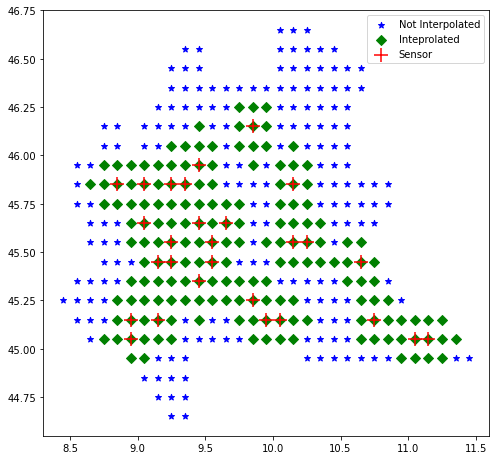
\includegraphics[scale=0.45]{images/buffer.png}}
 { \caption{Graphical representation of how buffer values interpolated from PM2.5 sensors provided by ARPA are added through k-nearest neighbour.}}
\end{figure}
\section{Feature Selection}
In this phase, I got the list of the most significant variables for each different configuration.
For doing that, after the features are selected for each period, an average of them is performed using again Borda Count algorithm. What is obtained is a general set of variables for each different configuration.
This was computed by averaging the feature selected for each different period with Borda Count another time;
Since I assume 2 different resolution and with the possibility to include or not the mountain zones, I obtained 4 different configurations: (TODO)
\begin{table}[H]
    \centering
    \begin{tabular}{|l|}
    \hline
        10km resolution (0.1°) with all clim\_zone (zone pedoclimatiche)  \\ \hline
        10km resolution (0.1°) without Alpes and Prealpes (clim\_zone > 3) \\ \hline
        1km resolution (0.01°) with all clim\_zone (zone pedoclimatiche)   \\ \hline
        1km resolution (0.01°) without Alpes and Prealpes (clim\_zone > 3)  \\ \hline
 
    \end{tabular}
\end{table}
In the \ref{fig:test_params} is shown a summary of the parameter of each test execution.
It can be observed that for each parameter there are different configurations: there are 2 resolutions, 2 climate zones parameter and 5 periods. Thus, for each different target variable, have been run 2x2x5 = 20 different tests both for ammonia and fine particulate (40 in total). 
Results from different periods for simplicity are grouped and averaged. In total in this work are attached 8 different results. Each results will be in detail pointed in the final Appendix TODO.
\begin{figure}[H]
    \centering
    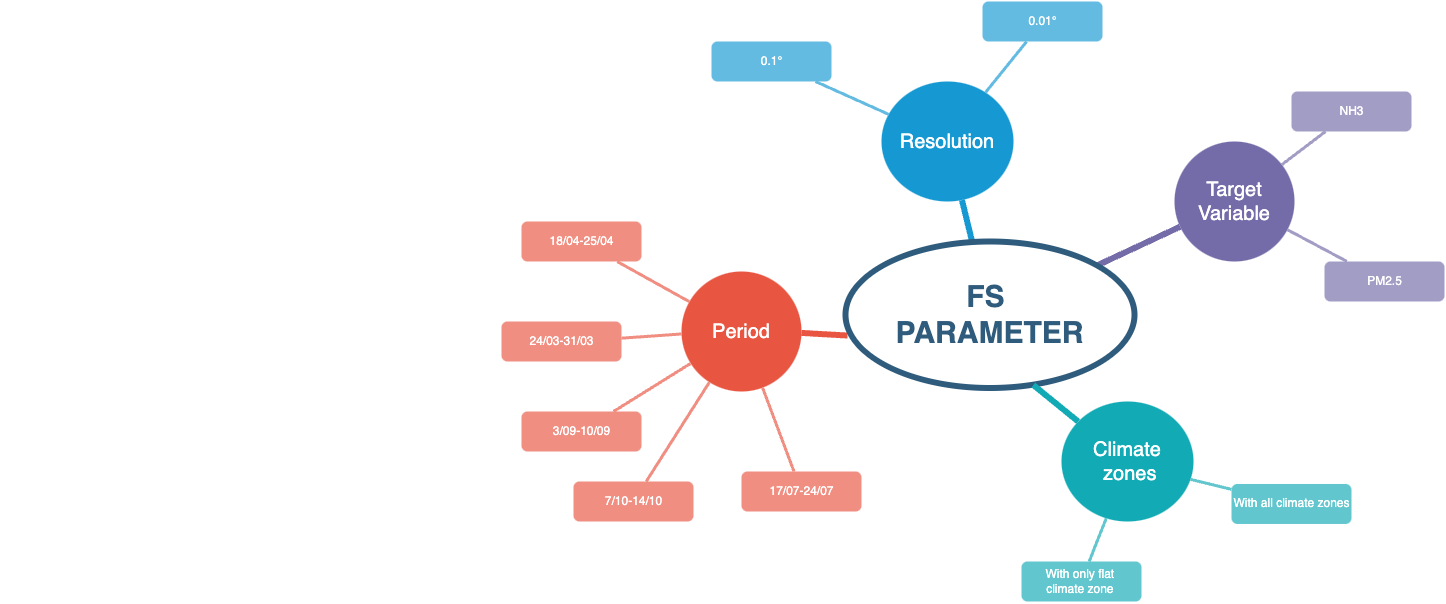
\includegraphics[width=.9\textwidth]{images/test_param.png}
    \caption{Parameter taken in consideration for tests execution.}
    \label{fig:test_params}
\end{figure}


\section{Data Modelling}
After the evaluation of variable selected by each different configuration, models (already explained in the previous chapter) are built and a cross validation for error and accuracy is evaluated. The validation is taken using the test set from test set of the target variable. In addition, a validation with PM25 values assumed by the CAMS models is taken. The validation with CAMS results consists simply in a comparison between the results obtained and the values of the CAMS model.  
\newline
In this way, a comparison between results from these 2 different validations is performed, aiming to detect how much the models perform better in this local scale.\par

https://www.sciencedirect.com/topics/agricultural-and-biological-sciences/agricultural-pollution 
https://pure.iiasa.ac.at/id/eprint/14769/1/Reduction%20of%20NH3%20emissions%20from%20agriculture%20in%20the%20Hai%20River%20Basin%20in%20China.pdf

https://towardsdatascience.com/batch-mini-batch-stochastic-gradient-descent-7a62ecba642a